
In this thesis, all the simulations are based on the geometry of a skew quadrupole which belongs to the group of high-order corrector magnets designed for the upgrade of the High-Luminosity LHC. Skew quadrupole is developed by LASA laboratories of INFN-Milano. Its geometry is presented in Fig. \ref{fig:Skew_quad_geometry}. Its two half-quadrants of two separate quadrants are positioned in one mechanical support. The entire magnet is placed inside the iron yoke. 

\begin{figure}[h!]
    \centering
    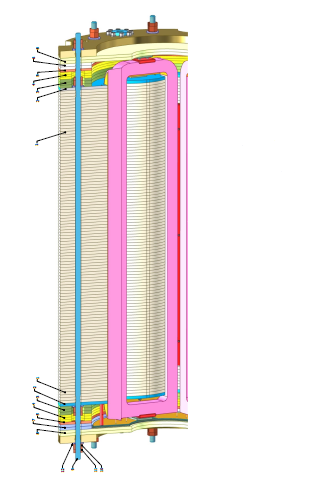
\includegraphics[width=0.25\linewidth]{sections/1D_quench_modelling/figures/geometry/SkewQuad3D.png}
    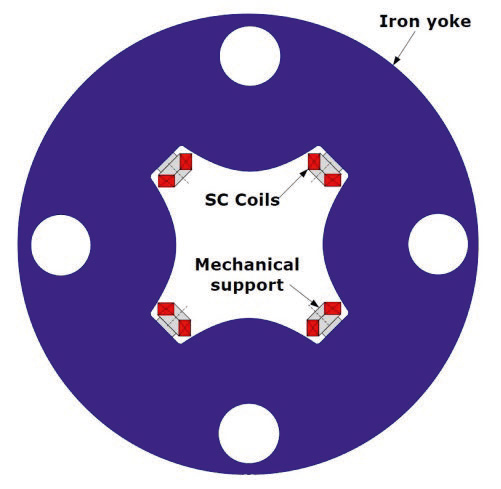
\includegraphics[width=0.30\linewidth]{sections/1D_quench_modelling/figures/geometry/Quadrupole_Cross_Section.png}
    \caption{Left: quarter of skew quadrupole 3D geometry; right: cross-section of skew quadrupole \cite{hl_lhc_tech_design_report_v01}}
    \label{fig:Skew_quad_geometry}
\end{figure}

Each quadrant of the magnet consists of 754 windings. The geometrical data input are collected and specified altogether in Table \ref{table:skew_quad_params_table}.

\begin{table}[h!]
    \caption{Geometrical parameters for skew quadrupole \cite{hl_lhc_tech_design_report_v01, marco_prioli_mails}} 
    \vspace{-1.em} 
    \fontsize{10}{10}
    \selectfont 
    \renewcommand{\arraystretch}{1.5}
    \begin{center}
    \begin{tabular}{ ccc }  
    \hline
    Aperture & 150 & [mm]\\
    Coil length & 841 & [m] \\
    Number of apertures & 1 & \\
    Number of circuits & 1 & \\
    Strand diameter & 0.7 & [mm] \\
    $\text{A}_\text{Cu}/\text{A}_\text{Nb-Ti}$ \cite{marco_prioli_mails} & 2.2 & \\
    \hline 
    \end{tabular}
    \end{center}  
     \label{table:skew_quad_params_table} 
 \end{table}





% Each cable is a single Nb-Ti strand of 0.7 mm diameter with a copper stabilizer. As presented in Fig. \ref{fig:materials_cross_section}, the winding is covered with 0.007 mm thick S2-glass insulation (in red). Then, the winding is immersed in epoxy resin D10 (in blue). The superconducting cable is marked in yellow. Moreover, ground insulation is added on the external side of the coil \cite{hl_lhc_tech_design_report_v01}.

% In the superconducting magnet design community, an assumption is often proposed to simulate the materials behaviour outside of the superconducting cable as a single domain characterized by the properties of G10 which is another material widely used in cryogenics. Such an assumption is made in this thesis. The characteristics of all material properties taken into consideration in the analysis are described in Appendix \ref{appendix_material_properties_description}.


% The stabilizer to superconductor ratio is specified in \cite{hl_lhc_tech_design_report_v01} and is calculated as follows:

